\documentclass{sig-alternate}
\usepackage[english]{babel}
\usepackage[utf8]{inputenc}
\usepackage[T1]{fontenc}
\usepackage{mathtools}
\usepackage{graphicx}
\usepackage{appendix}
\usepackage{hyperref}
\usepackage{color}

\newcommand{\equref}[1]{Equation~(\ref{#1})}
\newcommand{\figref}[1]{Figure~\ref{#1}}
\newcommand{\apref}[1]{Appendix~\ref{#1}}
\newcommand{\secref}[1]{Section~\ref{#1}}
\newcommand{\dindex}[3]{#1_{#2,\;#3}}

\newcommand{\note}[1]{\textcolor{red}{NOTICE: #1}}
\newcommand{\todo}[1]{\textcolor{blue}{TODO: #1}}


% \usepackage[sectionbib]{chapterbib}
\usepackage{multibib}
\newcites{app}{Appendix References}

% Remove the copyright
% \usepackage{etoolbox}
% \makeatletter
% \patchcmd{\maketitle}{\@copyrightspace}{}{}{}
% \makeatother

% Change the title font and spacing
\newfont{\titlefont}{phvb8t at 17pt}
\newfont{\authornamefont}{phvr8t at 12pt}
\newfont{\universityfont}{phvr8t at 10pt}
\newfont{\countryfont}{phvr8t at 10pt}
\newfont{\authoremailfont}{phvr8t at 12pt}

\newcommand{\authorname}[1]{{\authornamefont #1}}
\newcommand{\university}[1]{{\universityfont #1}}
\newcommand{\country}[1]{{\countryfont #1}}
\newcommand{\authoremail}[1]{{\authoremailfont #1}}

\makeatletter
\renewcommand{\@maketitle}{
  \newpage
  \null
  % \vskip 2em%
  \begin{center}%
    {\titlefont \@title \par}%
    \vspace{1.5em}
    {\@author \par}%
  \end{center}%
  \par%
  \vspace{14pt}%
}
\makeatother

\begin{document}
  \conferenceinfo{DAC}{'12 San Francisco, California, USA}
  \CopyrightYear{2012}
  % \crdata{}

  \title{Steady-State Dynamic Temperature Analysis and Reliability Optimization for Embedded Multiprocessor Systems}

  \numberofauthors{4}
  % \author{
  %   \alignauthor
  %     Ivan Ukhov\\
  %     \affaddr{Link\"{o}ping University}\\
  %     \affaddr{Sweden}\\
  %     \email{ivan.ukhov@liu.se}
  %   \alignauthor
  %     Min Bao\\
  %     \affaddr{Link\"{o}ping University}\\
  %     \affaddr{Sweden}\\
  %     \email{min.bao@liu.se}
  %   \alignauthor
  %     Petru Eles\\
  %     \affaddr{Link\"{o}ping University}\\
  %     \affaddr{Sweden}\\
  %     \email{petru.eles@liu.se}
  %   \alignauthor
  %     Zebo Peng\\
  %     \affaddr{Link\"{o}ping University}\\
  %     \affaddr{Sweden}\\
  %     \email{zebo.peng@liu.se}
  % }
  \author{
    \begin{tabular}[t]{@{\extracolsep{14pt}}cccc}
      \authorname{Ivan Ukhov} & \authorname{Min Bao} & \authorname{Petru Eles} & \authorname{Zebo Peng} \\
      \university{Link\"{o}ping University} & \university{Link\"{o}ping University} & \university{Link\"{o}ping University} & \university{Link\"{o}ping University} \\
      \country{Sweden} & \country{Sweden} & \country{Sweden} & \country{Sweden} \\
      \authoremail{ivan.ukhov@liu.se} & \authoremail{min.bao@liu.se} & \authoremail{petru.eles@liu.se} & \authoremail{zebo.peng@liu.se}
    \end{tabular}
  }

  \date{July 3--7, 2012}

  \maketitle

  \begin{abstract}
    In this paper we propose an analytical technique for the steady-state dynamic temperature analysis of multiprocessor systems with periodic applications. The approach is accurate and fast enough to be included inside an optimization loop for embedded system design. Using the proposed solution, a temperature-aware reliability optimization based on the thermal cycling failure mechanism is performed. The experimental results show that the lifetime of an embedded system can significantly be improved without sacrificing its energy efficiency by taking into consideration the steady-state dynamic temperature profile of the system during the design stage.

  \end{abstract}

  % http://www.acm.org/about/class/how-to-use
  % http://www.acm.org/about/class/ccs98-html
  \vspace{-5pt}
  \category{C.3}{Special-Purpose and Application-Based Systems}{Microprocessor/microcomputer applications, real-time and embedded systems}
  \category{G.1.3}{Numerical Linear Algebra}{Sparse, structured, and very large systems}
  \category{G.3}{Probability and Statistics}{Reliability and life testing}
  \category{J.6}{Computer-Aided Engineering}{Computer-aided design.}

  % http://www.acm.org/about/class/1998
  \vspace{-5pt}
  \terms{Algorithms, Design, Performance, Reliability.}

  % Capitalized
  \vspace{-5pt}
  \keywords{Multicore, Temperature Analysis, Leakage Power.}

  \isection{Introduction and Prior Work}
  \subsection{Temperature Variation}
Morden policies for prevening temperature runaways and decreasing energy consumption, within such tecniques as dynamic power management (DPM) and dynamic voltage and frequency scaling (DVFS), keep puzzling embedded system architects with a constantly increasing strength. These and similar approaches may cause considerable temperature fluctuations within a multiprocessor system-on-chip (MPSoC), therefore, dramatically decreasing its reliability \cite{mihic2004}, \cite{simunic2005}.

The importance of the temperature distribution over ICs has been widely studied in the literature \cite{lu2004}. Hence, a large number of different methods for performance and energy optimization imposes the maximal temperature constrain. In this essence, the need of fast and accurate methods for obtaining temperature profiles becomes urgent.

In this paper we consider the HotSpot thermal model \cite{huang2006} and propose an extremely fast way to calculate the steady-state dynamic temperature curve (SSDTC) of an embedded system that executes a set of periodic tasks.

In order to demonstrate our approach, we perform the energy optimization with a constrain on the spatial temperature gradient within a die. The constrain is satisfied with the help of SSDTC that delivers the diapason of the temperature fluctuation. The optimization problem is solved through the mapping and scheduling based on genetic algorithms and the list scheduler described in \cite{schmitz2004}.

\subsection{A Motivational Example}
TODO.


  \isection{Architecture, Power, and\\Thermal Models} \label{sec:preliminaries}
  \label{sec:architecture-model}
We consider a heterogeneous multicore architecture with a set of processing elements $\Pi$ defined as the following:
\[
  \Pi = \{ \pi_i = (V_i, \: f_i, \: N_{gate \: i}): \; i = \range{0}{N_p - 1} \}
\]
where $V_i$, $f_i$, and $N_{gate \: i}$ are the supply voltage, frequency, and number of gates \cite{liao2005} of the $i$th core, respectively.

\label{sec:power-model}
The total power dissipation of a processing element is defined as the sum of the dynamic and leakage power: $P = P_{dyn} + P_{leak}$. The dynamic part is modeled as $P_{dyn} = C_{eff} \cdot f \cdot V^2$ where $C_{eff}$ is the effective switched capacitance, $V$ and $f$ are the supply voltage and frequency, respectively. The leakage part of the power dissipation is defined as \cite{liao2005}:
\begin{equation} \label{eq:total-power}
  P_{leak}(T) = N_{gate} \: V \: I_0 \left[ A \: T^2 e^{\frac{\alpha \: V + \beta}{T}} + B e^{(\gamma \: V + \delta)} \right]
\end{equation}
where $T$ and $V$ are the current temperature and supply voltage, respectively, $N_{gate}$ is the number of gates in the circuit, $I_0$ is the average leakage current at the reference temperature and supply voltage. $A$, $B$, $\alpha$, $\beta$, $\gamma$, and $\delta$ are the technology dependent constants found in \cite{liao2005}.

\label{sec:thermal-model}
Our proposed technique is based on the RC thermal model that employs the analogy between electrical and thermal circuits \cite{kreith2000}. Heat transfer is modeled with the following system of differential equations:
\begin{equation} \label{eq:fourier-model}
  \m{C} \: \frac{d\v{T}(t)}{dt} + \m{G} \: (\v{T}(t) - \v{T}_{amb})= \v{P}(t)
\end{equation}
where $\v{T}$ is the temperature vector, $\v{T}_{amb}$ is the ambient temperature vector, $\m{C}$ is the thermal capacitance matrix, $\m{G}$ is the thermal conductance matrix, and $\v{P}$ is the power dissipation vector. The dimensions of the system are $N_n \times N_n$, where $N_n$ is the number of nodes in the equivalent RC thermal circuit, which is further discussed in \appref{ap:thermal-circuits}.


  \isection{Problem Formulation} \label{sec:problem}
  Consider a multicore system that consists of $N_p$ processing elements $\Pi = \{ \pi_i: i = \range{0}{N_p - 1} \}$ and executes a periodic application with a period $\period$. We construct an equivalent RC thermal circuit of the system that contains $N_n$ thermal nodes. The dynamic power profile of the system is sampled into $N_s$ time intervals of duration $\Delta t$, called sampling interval, in such a way that the dynamic power dissipation and temperature of each node are assumed to be constant within an interval. The discrete dynamic power profile is defined as $\mathbb{P}_{dyn} \eqdef \{ P_{ij}: \: i = \range{0}{N_s - 1}; \: j = \range{0}{N_n - 1} \}$ where $P_{ij}$ is the dynamic power dissipation during the $i$th time interval of the $j$th thermal node. After the steady state is reached, the corresponding temperature profile becomes periodic and is defined as $\mathbb{T} \eqdef \{ T_{ij}: \: i = \range{0 }{N_s - 1}; \: j = \range{0}{N_n - 1} \}$ where $T_{ij}$ is the temperature of the $j$th node in the $i$th time interval. The profile is called the steady-state dynamic temperature profile (SSDTP).

\statement{Given}:
\begin{ilist}
  \item A multicore system with a set of processing elements $\Pi$ executing a periodic application.
  \item The discrete dynamic power profile $\mathbb{P}_{\:dyn}$ of the system\footnote{Power dissipation of inactive nodes, i.e., the nodes that belong to the thermal package, is zero.} with the sampling interval $\Delta t$.
  \item The floorplan of the chip corresponding to the level of details at which the thermal modeling is performed.
  \item The configuration of the thermal package, i.e., dimensions of the thermal interface material, heat spreader, and heat sink.
  \item The thermal parameters of the die and package, e.g., the thermal conductivity and thermal capacitance.
\end{ilist}

\statement{Find}:
\begin{ilist}
  \item The corresponding periodic temperature profile $\mathbb{T}$ of the system when the steady state is reached.
\end{ilist}
% Reasonable requirements for a solution are speed and accuracy, since the temperature analysis is often a part of an intensive optimization procedure where the SSDTP is to be computed thousands of times. Such a problem is described in \secref{sec:reliability}.


  % \vfill\eject
  \isection{State of the Art Solutions} \label{sec:hotspot-solution}
  \subsection{Iterative Simulation} \label{sec:hotspot-iterative-solution}
A rough approximation of the SSDTP can be obtained by running a temperature simulator over successive periods of the application until it can be assumed that the system has reached the thermal steady state. The simulator performs the transient temperature analysis where the common approach is to solve \equref{eq:fourier-model} numerically, for instance, using the fourth-order Runge-Kutta method \cite{press2007}.

The number of iterations required to reach the SSDTP depends on the thermal characteristics of the system. In order to illustrate this aspect, we have considered an application with the period of 0.5 $s$ running on five hypothetical platforms with core areas between 1 and 25 $mm^2$. The configuration of the die and thermal package can be found in the appendix (\tabref{tab:parameters}). We have run the temperature simulation with HotSpot \cite{huang2003} for 50 successive periods. The temperature profile in each period has been compared with the actual SSDTP, obtained with our analytical approach (\secref{sec:analytical-solution}), and the normalized root mean square error (NRMSE) has been calculated. The result is shown in \figref{fig:hotspot-error}. It can be observed that the number of successive periods over which the temperature simulation has to be performed, in order to achieve a satisfactory level of accuracy, is significant for the majority of configurations. For a 9 $mm^2$ die, for example, after 15 iterations, the NRMSE is still close to 20\%. This leads to large computational times, making it difficult to apply the technique inside an intensive optimization loop.

\subsection{Steady-State Approximation (SSA)} \label{sec:steady-state-approximation}
An approximation of the SSDTP has been proposed in \cite{huang2009}. Instead of solving the system of equations in \equref{eq:fourier-model}, it is assumed that during each time interval $\Delta t_i$, in which the power is constant, the system stays in its steady state. The derivative $d\v{T}/dt = 0$ and temperature can be calculated as $\v{T}_i = \m{G}^{-1} \v{P}_i$. The result is a stepwise temperature curve where each step corresponds to the steady-state temperature $\v{T}_i$ that would be reached if the constant power $\v{P}_i$ was applied for a sufficiently long time.

An example of such an approximation (SSA) along with the corresponding SSDTP for an application with 10 tasks and period of 0.1 $s$ is given in \figref{fig:steady-state-approximation}. The die area is 25 $mm^2$, the configuration of the chip is the same as in \tabref{tab:parameters}. The reduced accuracy of the SSA is due to the mismatch between the actual temperature within each interval $\Delta t_i$ and the hypothetical steady-state temperature. The inaccuracy depends on the thermal characteristics of the respective platform and on the application itself. To illustrate this, we have generated five applications with periods between 0.01 and 1~$s$ and computed approximated SSDTPs for die areas between 1 and 25 $mm^2$. The NRMSE relative to the correct SSDTP is shown in \figref{fig:steady-state-error}. It can be seen that, e.g., for a die area of 10 $mm^2$ and a period of $100~ms$ the NRMSE with the SSA is close to 40\%.


  \isection{Analytical Solution} \label{sec:analytical-solution}
  As it was shown in \secref{sec:hotspot-solution}, the state of the art solutions either produce inaccurate and, in extreme cases, completely useless results, or they are unacceplably slow. In this section we eliminate the first problem by obtaining an analytical expression of the SSDTP and tackle the second one in \secref{sec:condensed-equation} where a fast technique to perform the computations is proposed.

In the onwards explanation, without loss of generality, we assume $\v{T}(t) \equiv \v{T}(t) - \v{T}_{amb}$. Let the power consumption vector $\v{P}(t)$ be constant and equal to $\v{P}$, then the system given by \equref{eq:fourier-model} is a system of ordinary differential equations (ODE) with the following solution:
\begin{equation} \label{eq:solution}
  \v{T}(t) = e^{\m{A} t} \; \v{T}_0 + \m{A}^{-1}(e^{\m{A} t} - \m{I})\m{C}^{-1} \v{P}
\end{equation}
where $\m{A} = -\m{C}^{-1} \: \m{G}$ and $\v{T}_0$ is the initial temperature. Therefore, given a discrete power profile, the corresponding temperature profile can be found using the following recurrence:
\begin{equation} \label{eq:recurrent-system}
  \v{T}_{i+1} = \m{K}_i \: \v{T}_i + \m{B}_i \: \v{P}_i
\end{equation}
where:
\begin{align*}
  & \m{K}_i = e^{\m{A} \Delta t_i} \\
  & \m{B}_i = \m{A}^{-1}(e^{\m{A} \Delta t_i} - \m{I})\m{C}^{-1}
\end{align*}

\subsection{Transient Temperature Analysis}
Given the initial temperature $\v{T}_0$, the recurrence in \equref{eq:recurrent-system} can be applied to perform the TTA. Our experiments show that in the case of equal time intervals, where $\m{K}_i$ and $\m{B}_i$ are constants, this approach demonstrates a significant performance improvement relative to iterative solutions of ODEs, e.g., the fourth-order Runge-Kutta method implemented in HotSpot. The same observation is made in \cite{thiele2011}.

The TTA using the analytical technique given in \equref{eq:recurrent-system} can be employed to approximate the SSDTP as it is described in \secref{sec:hotspot-iterative-solution} dramatically speeding up the computational process. However, the number of required simulations is unchanged since it is basically an alternative way to perform the same type of analysis. The technique that we shall propose later on equals to only two simulations using the above-mentioned analytical approach while the produced solutions are exact.

\subsection{Steady-State Dynamic Temperature Analysis}
For the steady-state case the following system of linear equations can be derived from \equref{eq:recurrent-system}:
\[
  \begin{cases}
    \m{K}_0 \: \v{T}_0 - \v{T}_1 & = -\m{B}_0 \: \v{P}_0 \\
    ... \\
    -\v{T}_0 + \m{K}_{N_s - 1} \: \v{T}_{N_s - 1} & = -\m{B}_{N_s - 1} \: \v{P}_{N_s - 1}
  \end{cases}
\]
where the last equation respects the boundary condition and ensures the equality of temperature values on both ends of the overall period:
\begin{equation} \label{eq:boundary-condition}
  \v{T}_0 = \v{T}_{N_s}
\end{equation}
To get the whole picture, the system can be written as:
\begin{align}
  & \mathbb{K} \: \mathbb{X} = \mathbb{B} \label{eq:system} \\
  & \mathbb{K} = \left[
    \begin{array}{ccccc}
      \m{K}_0 & -\m{I} & 0 & \cdots & 0 \\
      0 & \m{K}_1 & -\m{I} &  & \vdots \\
      \vdots &  & \ddots & -\m{I} & 0 \\
      0 &  &  & \m{K}_{N_s - 2} & -\m{I} \\
      -\m{I} & 0 & \cdots & 0 & \m{K}_{N_s - 1}
    \end{array}
  \right] \nonumber \\
  & \mathbb{X} = \left[
    \begin{array}{c}
      \v{T}_0 \\
      \vdots \\
      \v{T}_{N_s - 1}
    \end{array}
  \right] \nonumber \\
  & \mathbb{B} = \left[
    \begin{array}{c}
      -\m{B}_0 \: \v{P}_0 \\
      \vdots \\
      -\m{B}_{N_s - 1} \: \v{P}_{N_s - 1}
    \end{array}
  \right] \nonumber
\end{align}
where $\mathbb{K}$ is a $N_n N_s \times N_n N_s$ matrix, $\mathbb{X}$ and $\mathbb{B}$ are vectors with $N_n N_s$ elements.

It can be seen that we have obtained a regular system of liner equations with a specific structure. Now we shall briefly discuss possible alternatives to solve it.

\subsubsection{Direct Dense Solutions}
The first straight-forward way to solve the system is to use dense solvers such as the LU decomposition. The problem here is that such systems could be extremely large, especially when we want to achieve a higher level of accuracy and, therefore, the power profile contains a lot of steps $N_s$. Each new step produces $N_n$ new equations in the system given by \equref{eq:system}. The complexity grows very rapidly with the number of processing elements $N_p$. For instanse, the simpliest model implemented in HotSpot uses the following relation:
\[
  N_n = 4 \times N_p + 12
\]
Therefore, each new processing element increases each matrix $K_i$ by 4 rows and 4 columns, and each vector $Y_i$ and $Q_i$ by 4 elements. As an example, if the power profile for a single-processor system is composed of 1000 steps, then having the same discretization but with one additional core results in a linear system with 4000 additional equations. All in all, a fast and accurate approach to solve \equref{eq:system} is required.


\subsubsection{Direct Sparse Solutions}
\image{sparseness-of-system}{80 210 80 210}{Sparseness of the system of linear equations for the SSDTP calculation. Each blue point corresponds to a non-zero element of the matrix of the system.}
One may notice that the matrix $\mathbb{A}$ is an extremely sparse matrix with a very specific structure that can be observed in \figref{fig:sparseness-of-system}. The matrix has non-zero elements only on its block diagonal (composed of $N_n \times N_n$ matrices), one subdiagonal just above the block diagonal, and one subdiagonal in the left bottom corner. Therefore, instead of the dense LU decomposition we can apply algorithms that are specially designed for such cases.
In our experiments we use the UMFPACK library, a set of routines for solving unsymmetric sparse linear systems based on the Unsymmetric MultiFrontal method (UMF) \cite{umfpack2004}.


\subsubsection{Solutions for Toeplitz and Block-Circulant Systems}
One can notice that the overall matrix of the system under the assumption of the equal time intervals becomes a block Toeplitz matrix, because inner blocks $\mathbb{A}(i, \: j)$ satisfy the following criterion:
\[
  \mathbb{A}(i, j) = \mathbb{A}(i+1, \: j+1), \; i, j = 0 \dots N_s - 2
\]

To be more specific, the matrix is a block-circulant matrix where each block row vector is rotated one block element to the right relative to the preceding block row vector. This leads us to a wide range of possible techniques to solve \mbox{$\mathbb{A} \: \mathbb{Y} = \mathbb{B}$}, for example, the Fast Fourier Transform (FFT) \cite{mazancourt1983}, \cite{vescovo1997}.

In spite of the fact that the FFT approach is \emph{much faster} then the solution obtained with the UMF, our experiments have shown that the condensed equation method is even faster (see \secref{sec:results-ssdtp}), therefore, we concentrate on it and discuss the FFT in brief as a possible alternative.

$\mathbb{A}$ has $N_s \times N_s$ blocks, each block is a $N_n \times N_n$ submatrix. Since the matrix is a block-circulant matrix, it can be represented with only $N_s$ blocks that form the top block row:
\[
  \mathbb{A}(j), \; j = 0 \dots N_s - 1
\]
and all other rows can be easily found shifting this one. To solve the system, we need to apply the Discrete Fourier Transform to these $N_s$ blocks:
\[
  \mathbb{A}(k)^f = \sum_{j = 0}^{N_s - 1} \mathbb{A}(j) \; \omega_{N_s}^{jk}, \; k = 0 \dots N_s - 1
\]
where $\omega_{N_s} = e^{\frac{-2 \pi i}{N_s}}$. Here we perform a bulk transform of all $N_n \times N_n$ vectors at once, whereas the vector-by-vector version is the following for each $n$ and $m = 0 \dots N_n - 1$:
\[
  \mathbb{A}(k)^f_{nm} = \sum_{j = 0}^{N_s - 1} \mathbb{A}(j)_{nm} \; \omega_{N_s}^{jk}, \; k = 0 \dots N_s - 1
\]
Note that in our case only two matrices are non-zero, therefore, this procedure can be shrunk. By applying the transformation, we come from the time domain to the frequency domain. Also we need to perform the same operation on the right-hand vector $\mathbb{B}$ splitted into $N_s$ chunks, denoted $\mathbb{B}(j)$, of $N_n$ successive elements:
\[
  \mathbb{B}(k)^f = \sum_{j = 0}^{N_s - 1} \mathbb{B}(j) \; \omega_{N_s}^{jk}, \; k = 0 \dots N_s - 1
\]

The next step is to solve $N_s$ systems with matrices $(\mathbb{A}(k)^f)^{\ast}$ and corresponding vectors $\mathbb{B}(k)^f$, the asterisk here denotes the complex conjugate:
\[
  (\mathbb{A}(k)^f)^{\ast} \; \mathbb{Y}(k)^f = \mathbb{B}(k)^f, \; k = 0 \dots N_s - 1
\]
where all matrices $\mathbb{A}(k)^f$ ($N_n \times N_n$ matrices) are symmetric, since $\mathbb{A}(k)$ are so, therefore, the eigenvalue decomposition can significantly simplify the solution process.

The last step is to return back to the time domain with the Inverse Discrete Fourier Transform:
\[
  \mathbb{Y}(k) = \frac{1}{N_s} \sum_{j = 0}^{N_s - 1} \mathbb{Y}(j)^f \; \omega_{N_s}^{-jk}, \; k = 0 \dots N_s - 1
\]


\subsubsection{Iterative Methods for Systems of Linear Equations}
Another possible technique is iterative methods for solving systems of linear equations (e.g., the Jacobi, Gauss–Seidel, Successive over-relaxation methods). These methods are designed to overcome problems of direct solvers, since they do not operate on full matrices and, therefore, consume less memory. Consequently, they can be applied for extremely large systems, but the most important issues with these methods are their convergence and accuracy. In our analysis we did not observe any advantages of using this methods for this particular problem, they demonstrated slow convergence and poor accuracy. Hence, we excude them from the paper.



  \isection{Proposed Technique} \label{sec:condensed-equation}
  In this section we propose a fast approach to solve the system given by \equref{eq:system}. The approach consists of an auxiliary transformation (\secref{sec:ce-auxiliary}) and the solution itself (\secref{sec:ce-solution}).

The major problem with the earlier-discussed techniques is that (1) the sparseness of the matrix is not taken into account, leading to an enormous memory consumption and prohibitive solutions, and/or (2) its specific structure, which is discussed later, is totally ignored, resulting in an inefficiency of the computations and inaccuracy. Our proposed technique considers both features and delivers solutions in time proportional to $N_s N_n^3$ while operating only on a few $N_n \times N_n$ matrices. The dependency on the number of steps in the power profile $N_s$, which it typically by far dominats, i.e., $N_s \gg N_n$, is linear. The preparatory work, needed by the technique, is done only once for a particular RC thermal circuit and can be considered as a given for various power profiles, which is not always the case with the other solutions.

\iimage{sparseness-of-system}{-60 210 -60 210}{Sparseness of the system of linear equations for the SSDTP calculation.}

Let us start with from the discussion on the above-mentioned specific structure, which importance is immense, of the system given by \equref{eq:system} and depicted in \figref{fig:sparseness-of-system}. It can be seen that non-zero elements, marked with blue points in the figure, are located only on the block diagonal, one subdiagonal just above the block diagonal, and one subdiagonal in the left bottom corner. The block diagonal is composed of $N_n \times N_n$ matrices while all elements of the subdiagonals are equal \mbox{to $-1$}. Linear systems with the same structure arise in boundary value problems for ODEs where a common technique to solve them is to form a so-called condensed equation (CE), or condensed system \cite{stoer2002}. Before undertaking this procedure, we perform an adjustment to the initial analytical solution described in the following subsection.

\subsection{Auxiliary Transformation} \label{sec:ce-auxiliary}
It can be noticed that the analytical solution in \equref{eq:solution} includes two computationally expensive operations, namely the matrix exponential and inverse involving \mbox{$\m{A} = - \m{C}^{-1} \: \m{G}$}, which is an arbitrary square matrix. It is preferable to have a symmetric matrix to perform these computations, since for a real symmetric matrix $\m{M}$ the following eigenvalue decomposition with independent eigenvectors holds \cite{press2007}:
\begin{equation} \label{eq:eigenvalue-decomposition}
  \m{M} = \m{U} \m{\Lambda} \m{U}^\v{T}
\end{equation}
where $\m{U}$ is a square matrix of the eigenvectors, $\m{U}^T$ is the transpose of $\m{U}$, and $\m{\Lambda}$ is a diagonal matrix of the eigenvalues of $\m{M}$. Once we have obtained such a decomposition, the calculation of the matrix exponential and inverse becomes a trivial task:
\begin{align*}
  & e^\m{M} = \m{U} \; e^{\m{\Lambda}} \; \m{U}^\v{T} = \m{U} \: \diag{e^{\lambda_0}}{e^{\lambda_{n - 1}}} \: \m{U}^\v{T} \\
  & \m{M}^{-1} = \m{U} \: \m{\Lambda}^{-1} \: \m{U}^\v{T} = \m{U} \: \diag{\frac{1}{\lambda_0}}{\frac{1}{\lambda_{n - 1}}} \: \m{U}^\v{T} \\
\end{align*}
where $diag$ denotes a diagonal matrix and $\lambda_i$ are eigenvalues of $\m{M}$.

The conductance matrix $\m{G}$ is a symmetric matrix, since if a node A is connected to B, then B is also connected to A with the same conductance \cite{huang2003}. However, as it is mentioned previously, the product of $\m{G}$ with the inverse of the capacitance matrix $\m{C}$ does not have this property. We propose to use the following transformation in order to keep the desired symmetry:
\begin{equation} \label{eq:substitution}
  \tilde{\v{T}}(t) = \m{C}^{\frac{1}{2}} \v{T}(t) \hs \tilde{\m{A}} = -\m{C}^{-\frac{1}{2}} \m{G} \: \m{C}^{-\frac{1}{2}}
\end{equation}
where $\tm{A}$ is symmetric, since $\tm{A}^T = -(\m{C}^{-\half} \m{G} \m{C}^{-\half})^T = -(\m{C}^{-\half})^T \m{G}^T (\m{C}^{-\half})^T = \tilde{\m{A}}$. Note that the capacitance matrix $\m{C}$ is a diagonal matrix \cite{huang2003}, hence, $\m{C}^\half$ takes linear time to compute. Consequently, the system of ODEs (\equref{eq:fourier-model}) and its solutions (\equref{eq:solution}) can be rewritten as the following:
\begin{align*}
  & \frac{d\tilde{\v{T}}(t)}{dt} = \tilde{\m{A}} \: \m{Y}(t) + \m{C}^{-\frac{1}{2}} \v{P} \\
  & \tilde{\v{T}}(t) = e^{\tilde{\m{A}} t} \tilde{\v{T}}_0 + \tilde{\m{A}}^{-1} (e^{\tilde{\m{A}} t} - \m{I}) \m{C}^{-\frac{1}{2}} \v{P}
\end{align*}
where $\tilde{\m{A}}$ is a symmetric matrix. Therefore, in the case of, e.g., the matrix exponential we have:
\begin{equation} \label{eq:matrix-exponential}
  e^{\tm{A} t} = \m{U} \: e^{\m{\Lambda} t} \: \m{U}^T = \m{U} \: \diag{e^{t \lambda_0}}{e^{t \lambda_{N_n - 1}}} \: \m{U}^T
\end{equation}
where $\lambda_i$ are eigenvalues of $\tilde{\m{A}}$. A similar equation can be obtained for the matrix inverse.

The next step is to update the SSDTP system given in \equref{eq:recurrent-system}:
\begin{align}
  & \tv{T}_{i+1} = \tm{K}_i \: \tv{T}_i + \tm{B}_i \: \v{P}_i \label{eq:recurrent-equation} \\
  & \tm{K}_i = e^{\tm{A} \: \Delta t_i} \hs \tm{B}_i = \tm{A}^{-1} \left( e^{\tilde{\m{A}} \Delta t_i} - \m{I} \right) \m{C}^{-\frac{1}{2}} \nonumber
\end{align}
Using the eigenvalue decomposition, the last equation can be computed in the following way:
\begin{align*}
  \tilde{\m{B}}_i & = \m{U} \: \m{\Lambda}^{-1} \: \m{U}^T \left(\m{U} \: e^{\m{\Lambda} \Delta t_i} \: \m{U}^T - \m{U} \: \m{U}^T \right) \m{C}^{-\frac{1}{2}} = \\
  & = \m{U} \: \diag{\frac{e^{\Delta t_i \: \lambda_0} - 1}{\lambda_0}}{\frac{e^{\Delta t_i \: \lambda_{N_n - 1}} - 1}{\lambda_{N_n - 1}}} \: \m{U}^T \: \m{C}^{-\frac{1}{2}}
\end{align*}

\subsection{Solution with Condensed Equation (CE)} \label{sec:ce-solution}
Let us return back to the recurrent system given by \equref{eq:recurrent-equation} and denote \mbox{$\m{Q}_i = \tilde{\m{B}}_i \: \v{P}_i$}:
\begin{align}
  & \tilde{\v{T}}_{i + 1} = \tilde{\m{K}}_i \: \tilde{\v{T}}_i + \m{Q}_i, \; i = \range{0}{N_s - 1} \label{eq:ce-recurrent} \\
  & \tilde{\v{T}}_0 = \tilde{\v{T}}_{N_s + 1} \nonumber
\end{align}
In order to form the condensed equation mentioned in the beginning of this section, we perform the iterative repetition of \equref{eq:ce-recurrent} that leads us to:
\begin{equation} \label{eq:y-recurrent}
  \tv{T}_i = \prod_{j = 0}^{i - 1} \tm{K}_j \: \tv{T}_0 + \m{W}_{i - 1}, \; i = \range{1}{N_s}
\end{equation}
where $\m{W}_i$ are defined as the following:
\begin{align}
  \m{W}_0 & = \m{Q}_0 \nonumber \\
  %\m{W}_i & = \sum_{l = 1}^i \prod_{j = l}^i \tilde{\m{K}}_j \: \m{Q}_{l - 1} + \m{Q}_i, \: i = \range{1}{N_s - 1} \nonumber \\
  \m{W}_i & = \tm{K}_i \: \m{W}_{i - 1} + \m{Q}_i, \; i = \range{1}{N_s - 1} \label{eq:p-recurrent}
\end{align}
Therefore, we can calculate the final vector $\tilde{\v{T}}_{N_s}$ using \equref{eq:y-recurrent} and \equref{eq:p-recurrent}:
\[
  \tilde{\v{T}}_{N_s} = \prod_{j = 0}^{N_s - 1} \tilde{\m{K}}_j \: \tilde{\v{T}}_0 + \m{W}_{N_s - 1}
\]
Taking into account the boundary condition given by \equref{eq:boundary-condition}, we obtain the following system of linear equations:
\begin{equation} \label{eq:core-system}
  (\m{I} - \prod_{j = 0}^{N_s - 1} \tm{K}_j) \: \tv{T}_0 = \m{W}_{N_s - 1}
\end{equation}
We recall that $\tm{K}_i$ is the matrix exponential given by \equref{eq:matrix-exponential}, therefore, the following simplification holds:
\[
  \prod_{j = i}^l \tm{K}_j = \prod_{j = i}^l e^{\tm{A} \Delta t_j} = e^{\tm{A} \sum_{j = i}^l \Delta t_j} = \m{U} e^{\left( \sum_{j = i}^l \Delta t_j \: \m{\Lambda} \right)} \m{U}^T
\]
Consequently:
\[
  \prod_{j = 0}^{N_s - 1} \tm{K}_j = \m{U} \: \diag{e^{\period \lambda_0}}{e^{\period \lambda_{N_n - 1}}} \: \m{U}^T
\]
where $\period$ is the application period. Substituting this product into \equref{eq:core-system}, we obtain the following system:
\[
  (\m{I} - \m{U} \: e^{\period \m{\Lambda}} \: \m{U}^T) \: \tv{T}_0 = \m{W}_{N_s - 1}
\]
The identity matrix $\m{I}$ can be splitted into $\m{U} \m{U}^T$, hence:
\[
  \tv{T}_0 = \m{U} \: (\m{I} - e^{\period \m{\Lambda}})^{-1} \: \m{U}^T \: \m{W}_{N_s - 1} = \m{Z} \: \m{W}_{N_s - 1}
\]
where:
\begin{equation} \label{eq:m-matrix}
  \m{Z} = \m{U} \: \diag{\frac{1}{1 - e^{\period \lambda_0}}}{\frac{1}{1 - e^{\period \lambda_{N_n - 1}}}} \: \m{U}^T
\end{equation}
The equation gives the initial solution vector $\tv{T}_0$, the rest of vectors $\tv{T}_i$ for $i = \range{1}{N_s - 1}$ are successively found from \equref{eq:ce-recurrent}.

Since the power profile is evenly sampled with the sampling interval $\Delta t$, i.e., $\Delta t_i = \Delta t$ for $i = \range{0}{N_s - 1}$, the recurrent process in \equref{eq:recurrent-equation} turns into:
\[
  \tilde{\v{T}}_{i+1} = \tilde{\m{K}} \: \tilde{\v{T}}_i + \tilde{\m{B}} \: \v{P}_i
\]
where:
\[
  \tm{K} = e^{\tm{A} \: \Delta t} \hs \tm{B} = \tm{A}^{-1} ( e^{\tm{A} \: \Delta t} - \m{I} ) \m{C}^{-\frac{1}{2}}
\]
Here $\tm{K}$ and $\tm{B}$ are constants, since they depend only on the matrices $\tm{A}$, $\m{C}$, and sampling interval $\Delta t$, which is fixed. In this case, the block diagonal of the matrix $\tilde{\mathbb{A}}$, similar to \equref{eq:system}, is composed of the same repeating block $\tilde{\m{K}}$ and the recurrent expressions take the following form:
\begin{align}
  & \tv{T}_{i + 1} = \tm{K} \: \tv{T}_i + \m{Q}_i, \; i = \range{0}{N_s - 1} \nonumber \\
  & \m{W}_i = \tm{K} \: \m{W}_{i - 1} + \m{Q}_i, \; i = \range{1}{N_s - 1} \nonumber
\end{align}
The last step of the solution is to return back to temperature by performing the backward substitution opposite to \equref{eq:substitution}:
\[
  \v{T}_i = \m{C}^{-\frac{1}{2}} \: \tv{T}_i, \: i = \range{0}{N_s - 1}
\]

As we see, the auxiliary substitution from \secref{sec:ce-auxiliary} allows us to perform the single-time eigenvalue decomposition with orthogonal eigenvectors (\equref{eq:eigenvalue-decomposition}) that later eases the computational process at several stages. First, the decomposition is employed to compute the matrix exponential, matrix inverse, and, consequently, matrices $\tm{K}$ and $\tm{B}$. Then, the linear system given by \equref{eq:core-system} is solved without any explicit inversion of any matrix, the solution $\tv{T}_0$ is obtained by scalar divisions and a similarity transformation with $\m{U}$ (\equref{eq:m-matrix}).

As it was mentioned previously, the eigenvalue decomposition along with $\tm{K}$ and $\tm{B}$ are computed only once for a particular RC thermal circuit and can be considered as a given for optimization purposes, significantly decreasing the computational time. Moreover, if the subject of optimization is the same time interval, \equref{eq:m-matrix} is a constant as well.


  \isection{Leakage Power} \label{sec:leakage}
  \begin{figure*}
  \centering
  \begin{minipage}{0.30\linewidth}
    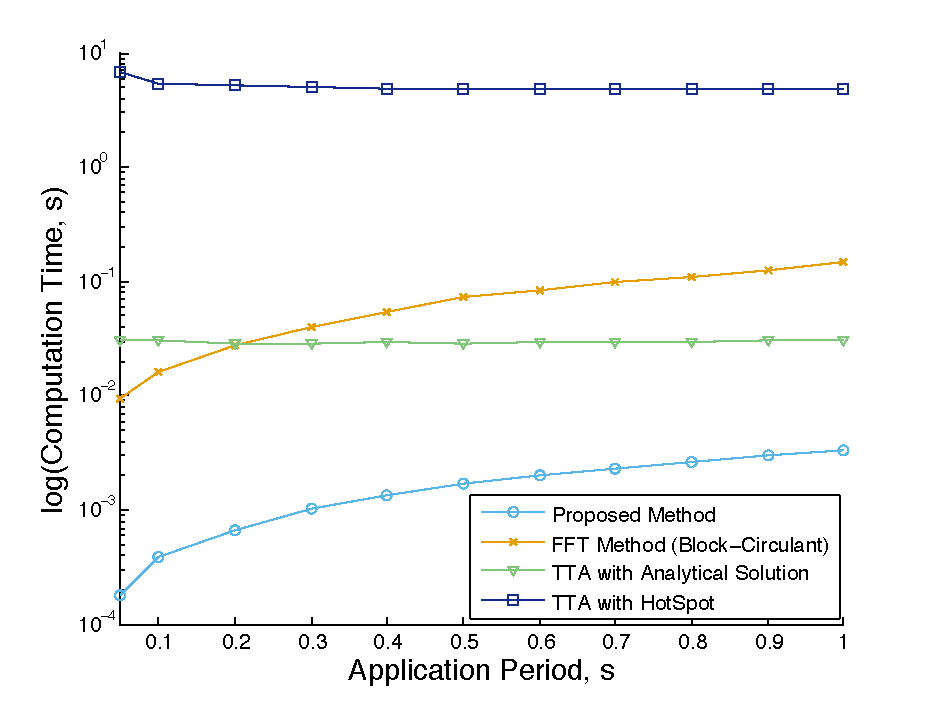
\includegraphics[clip=true, trim=15 0 15 0, width=\linewidth]{assets/scaling-time.pdf}
    \caption{Scalability with $\period$.}
    \label{fig:scaling-time}
  \end{minipage}
  \begin{minipage}{0.30\linewidth}
    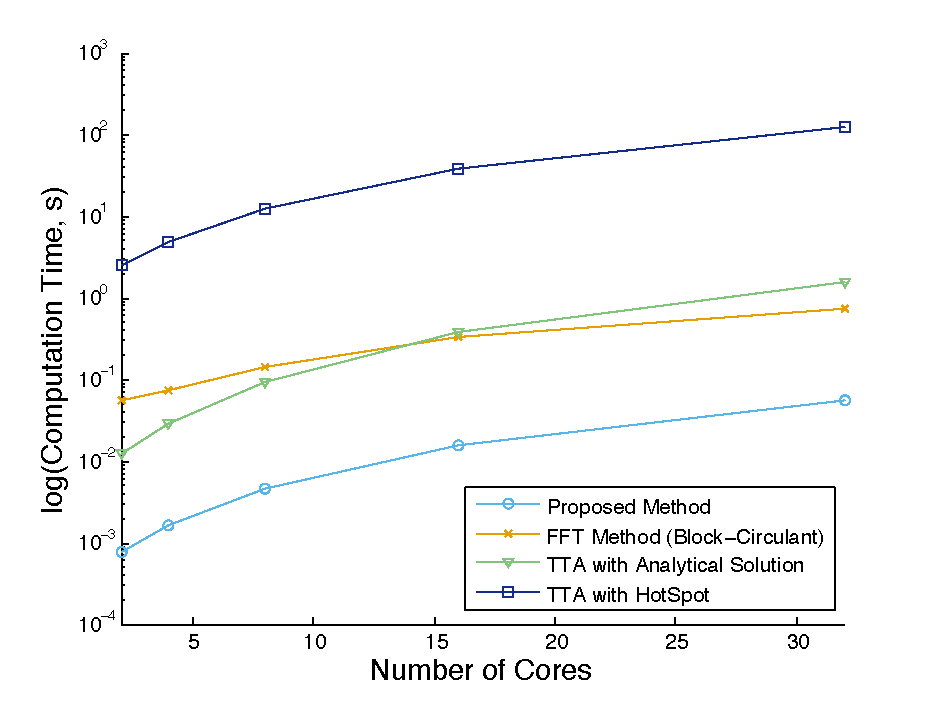
\includegraphics[clip=true, trim=15 0 15 0, width=\linewidth]{assets/scaling-cores.pdf}
    \caption{Scalability with $N_p$.}
    \label{fig:scaling-cores}
  \end{minipage}
  \begin{minipage}{0.35\linewidth}
    \includegraphics[clip=true, trim=50 0 50 0, width=\linewidth]{assets/average-pareto.pdf}
    \caption{Average Pareto front.}
    \label{fig:average-pareto}
  \end{minipage}
\end{figure*}

So far, we have assumed that power is independent of temperature. However, due to the leakage component, the power dissipation is a strong function of temperature that cannot be neglected (\secref{sec:power-model}). Two techniques can be applied to include in our proposed solution temperature dependent leakage modeling.

\subsection{Iterative Computation} \label{sec:iterative-leakage}
In this case, we have an iterative process, depicted in \figref{fig:leakage}, where the temperature and power profiles are calculated in turns. With each new temperature profile we update the power profile by computing the leakage power and adding it to the dynamic power: $\mathbb{P}_i = \mathbb{P}_{dyn} + \mathbb{P}_{leak}(\mathbb{T}_i)$. The process continues until the temperature converges, i.e., the difference between two successive temperature profiles is below a predefined bound. In our experiments we used $0.5^\circ C$ as the maximal acceptable difference and observed that the number of required iterations to converge is 4--7.

\subsection{Linear Approximation} \label{sec:linearized-leakage}
A linear approximation of the leakage power has the following matrix form: $\v{P}_{leak}(\v{T}) = \m{A} \: \v{T}(t) + \v{B}$ where $\m{A}$ is a $N_n \times N_n$ diagonal matrix of the proportionality and $\v{B}$ is a vector with $N_n$ elements of the intercept. Both characterize the leakage power for each of the $N_n$ thermal nodes in the system. It can be seen that the approximation keeps \equref{eq:fourier-model} untouched: $\m{C} \: \frac{d\v{T}(t)}{dt} + \bar{\m{G}} \: (\v{T}(t) - \v{T}_{amb}) = \bar{\v{P}}$ where $\bar{\m{G}} = \m{G} - \m{A}$ and $\bar{\v{P}} = \v{P}_{dyn} + \m{A} \: \v{T}_{amb} + \v{B}$. Therefore, all solutions proposed in this paper are perfectly valid with the linearized model. Moreover, in spite of its simplicity, the model provides a good estimation as shown in \cite{liu2007}.

In order to evaluate the linearization, we have constructed a number of hypothetical platforms with 2--32 cores (other parameters are given in \tabref{tab:parameters}) and compared temperature profiles obtained with the linearization and the exponential model (\secref{sec:power-model}), respectively. For the later, we use the iterative approach described above. For the linearization, the power curve fitting with the least squares regression \cite{press2007} has been employed, targeted at the range between 40 and $80^\circ C$. From the experiments we have observed that the NRMSE is bounded by 1--2\%, indicating a good accuracy of the linear approximation.


  \isection{Reliability Optimization} \label{sec:reliability}
  The proposed solution of the steady-state dynamic temperature estimation can be used in a wide range of optimization procedures. One of them is the reliability optimization that we discuss in this section. We performing the temperature-aware task mapping and scheduling in order to address the thermal cycling aging effect while keeping the energy consumption on an appropriate level. Both mapping and scheduling are based on the genetic algorithms \cite{schmitz2004}. Let us start with the overall description of the system.

\subsection{Application Model}
The system executes a periodic application with a set of data-dependent tasks. The overall structure of the application is defined by a task graph:
\begin{align*}
  & G = (\mathcal{V}, \: E, \: \mathcal{T}) \\
  & \mathcal{V} = \{ v_i: \: i = 0 \dots N_t - 1 \} \\
  & E = \{ e_{ij} \}
\end{align*}
where $\mathcal{V}$ is a set of $N_t$ vertices of the graph (tasks), $E$ is a set of edges (data dependencies between tasks), and $\mathcal{T}$ is the period of the application. Each pair of a task $v_i$ and processing element $\pi_j$ is characterized by a tuple $(C_{eff \; ij}, N_{cycles \; ij})$, where $C_{eff \; ij}$ is the effective switched capacitance and $N_{cycles \: ij}$ is the number of clock cycles. These parameters determine the processor load and execution time of the task, correspondingly.

\subsection{Temperature-Aware Reliability Model}
In the paper we address temperature-driven failure mechanisms with the reliability model presented in \cite{huang2009}, \cite{xiang2010}. The model is based on the assumption that the failure rate has a Weibull distribution (e.g., the thermal cycling, electromigration, etc. \cite{jedec2010}):
\[
  R(t) = e^{-(\frac{t}{\eta})^\beta}
\]
where $\eta$ is the scaling parameter, $\beta$ is the shape (slope) parameter. The mean time to failure (MTTF) for the Weibull distribution is given by the following equation:
\begin{equation} \label{eq:general-mttf}
  MTTF = \eta \; \Gamma(1 + \frac{1}{\beta})
\end{equation}
where $\Gamma$ is the gamma function. The shape parameter is found to be independent on the temperature variation \cite{chang2006}, which is not the case with the scaling parameter $\eta$. Therefore, the distribution can vary from one set of conditions to another. We can use the same approach as it was shown previously and split the overall period of the application $\mathcal{T}$ into $N_m$ time intervals $\Delta t_i$, so that during each time interval $\Delta t_i$ all those conditions can be treated as constants, consequently, the corresponding $\eta_i$ is also constant. In this case, the cumulative distribution function by the end of the first execution of the application is the following \cite{huang2009}, \cite{xiang2010}:
\[
  R = e^{-(\sum_{i=0}^{N_m - 1} \frac{\Delta t_i}{\eta_i})^\beta}
\]

It can be shown that if $\eta_i$ are large enough\footnote{This is the case, since usually the MTTF is in order of tens of years (see \equref{eq:general-mttf}).}, the following continuous approximation can be applied \cite{xiang2010}:
\[
  R(t) = e^{-(\frac{t}{\mathcal{T}} \sum_{i=0}^{N_m - 1} \frac{\Delta t_i}{\eta_i})^\beta}
\]
The formula still keeps the form of the Weibull distribution with the following scaling parameter:
\[
  \eta = \frac{\mathcal{T}}{\sum_{i=0}^{N_m - 1} \frac{\Delta t_i}{\eta_i}}
\]

As it was mentioned earlier, the reliability model can be used to model different failure mechanisms. Let us now focus on one particular failure cause, the thermal cycling (TC) fatigue, that is a common packaging and interfacial failure mechanism \cite{jedec2010}. The number of cycles to failure can be estimated using a modified version of the well-known Coffin-Manson equation with the Arrhenius term \cite{jedec2010}, \cite{xiang2010}, \cite{ciappa2003}:
\begin{equation} \label{eq:cycles-to-failure}
  \mathcal{N} = A (\Delta T - \Delta T_0)^{-b} e^{\frac{E_a}{k T_{max}}}
\end{equation}
where $A$ is an empirically determined constant, $\Delta T$ is the thermal cycle amplitude, $\Delta T_0$ is the portion of the temperature range in the elastic region which does not cause damage, $b$ is the Coffin-Manson exponent which also empirically determined\footnote{This constant is found to be 6--9 for brittle fracture such as Si and its dielectrics \cite{jedec2010}.}, $E_{a}$ is the activation energy\footnote{For the thermal cycling failure mechanism the activation energy lies between 0.5 and 0.7~eV \cite{vigrass}.}, $k$ is the Boltzmann constant, and $T_{max}$ is the maximal temperature during the thermal cycle. Having the number of cycles to failure and the duration of one cycle $\Delta t$, we can compute the MTTF:
\[
  MTTF = \mathcal{N} \; \Delta t
\]

Since we consider the TC failure mechanism, the time intervals $\Delta t_i$ correspond to intervals of constant parameters of this particular mechanism that can be observed on \equref{eq:cycles-to-failure}. Each interval $\Delta t_i$ belongs to one thermal cycle with the scaling parameter $\eta_i$ derived using \equref{eq:general-mttf}:
\[
  \eta_i = \frac{MTTF_i}{\Gamma(1 + \frac{1}{\beta})}
\]
where $MTTF_i$ is the mean time to failure of the $i$th time interval as if we had the failure distribution of this interval all the time. Taking everything together, we get the following equation:
\begin{equation} \label{eq:one-mttf}
  MTTF = \frac{\mathcal{T}}{\sum_{i=0}^{N_m - 1} \frac{1}{\mathcal{N}_i}}
\end{equation}

\equref{eq:one-mttf} describes the MTTF of one component, which is a processing element in our case. We assume that each processing element is essential for the proper work of the system, therefore, a failure of any core leads to the total failure of the whole system. Consequently, the MTTF of the system can be estimated as the minimal MTTF among its components:
\begin{align*}
  & MTTF_{sys} = \min_{i=0}^{N_p - 1} \; MTTF_i \\
  & MTTF_i = \frac{\mathcal{T}}{\sum_{j=0}^{N_{m \: i} - 1} \frac{1}{\mathcal{N}_{ij}}}
\end{align*}
where $N_{m \: i}$ is the number of thermal cycles of the $i$th processing element within the application period $\mathcal{T}$ and $\mathcal{N}_{ij}$ is the number of thermal cycles to failure as if the $j$th cycle was being repeated all the time.

\subsection{Motivational Example} \label{sec:motivation}
\iimage{task-graph}{0 0 0 0}{Motivational example with 6 tasks, labeled from ``T0'' to ``T5'', running on a heterogeneous dual-core architecture. The execution times of the tasks vary between cores and are given on the figure along with the period of the application.}
\image{motivation}{100 240 100 240}{Three alternative combinations of mapping and scheduling (the left side) of the application shown in \figref{fig:task-graph} onto a dual-core architecture and corresponding steady-state dynamic temperature curves (the right side) for each of the cores.}
Consider a toy application with six tasks, denoted ``T0''--``T5'', and a heterogeneous architecture with two cores, labeled ``PE0'' and ``PE1''. The task graph of the application is given in \figref{fig:task-graph}. The initial mapping, schedule, and resulting SSDTP are shown at the top of \figref{fig:motivation}, where PE0 is experiencing three thermal cycles. If we change the allocation of T5 and move it to PE1, we achieve two thermal cycles of PE0 instead of three. Finally, if we vary the schedule as well and change the order of T1 and T3, the number of cycles of PE0 becomes one. Using the reliability model from \secref{sec:reliability}, we observe improvements in the MTTF of 45\% and 54\%, respectively, relative to the initial configuration.



  \isection{Experimental Results} \label{sec:results}
  \subsection{Computation Performance} \label{sec:results-ssdtp}
In this subsection we investigate the scalability properties of the proposed solution for the SSDTP calculation and compare it with the approaches based on the FFT (\secref{sec:fast-fourier-transform}), TTA with the analytical solution (\secref{sec:tta-analytical}), and TTA with HotSpot (\secref{sec:hotspot-solution})\footnote{All the experiments are done on a Linux machine with Intel\textregistered\ Core\texttrademark\ i7-2600 (3.4GHz, 4 cores, 8 threads) and 8Gb of RAM.}. In the last two case, the TTA is run until the normalized RMSE relative to the SSDTP obtained with the CE method is less than 1\%. The sampling interval is equal to \mbox{1 $ms$}.

\subsubsection{Various Application Periods}
\iimage{scaling-time}{40 230 40 230}{Scalability with the application period for a quad-core architecture. The comparison is given on the semilogarithmic scale.}
\begin{itable}{scaling-time}{|r|r|r|r|r|r|r|}
  {Scalability with the application period shown in \figref{fig:scaling-time}.}
  {$\period$ --- application period, CE --- computational time of the CE method in $ms$, FFT --- speed-up relative to the FFT method, $TTA^{AS}$, $TTA^{HS}$ --- speed-up relative to the TTA with the analytical solution and TTA with HotSpot, respectively, along with the number of iterations.}
  \hline
  \multirow{2}{*}{$\period$, s} & \multirow{2}{*}{CE, ms} & \multirow{2}{*}{FFT, $\times$} & \multicolumn{2}{c|}{$TTA^{AS}$} & \multicolumn{2}{c|}{$TTA^{HS}$} \\ \cline{4-7}
  & & & $\times$ & Periods & $\times$ & Periods \\
  \hline
  \hline
  0.05 & 0.18 & 52.12 & 168.71 & 385 & 6750.96 & 689 \\
  0.10 & 0.39 & 41.64 &  77.91 & 191 & 5301.97 & 268 \\
  0.20 & 0.67 & 41.64 &  42.79 &  95 & 5188.80 & 122 \\
  0.30 & 1.03 & 39.09 &  27.97 &  63 & 5030.25 &  86 \\
  0.40 & 1.36 & 39.16 &  21.43 &  48 & 4887.90 &  63 \\
  0.50 & 1.70 & 43.56 &  16.99 &  38 & 4880.57 &  50 \\
  0.60 & 2.04 & 40.86 &  14.34 &  32 & 4899.20 &  42 \\
  0.70 & 2.32 & 42.46 &  12.87 &  28 & 4935.89 &  36 \\
  0.80 & 2.66 & 41.70 &  11.07 &  24 & 4842.62 &  31 \\
  0.90 & 2.98 & 42.54 &  10.21 &  22 & 4883.76 &  28 \\
  1.00 & 3.33 & 45.19 &   9.23 &  20 & 4892.86 &  25 \\
  \hline
\end{itable}
First, we vary the application period keeping the architecture fixed, which is a quad-core platform with the core area of 4 $mm^2$ and configuration shown in \tabref{tab:parameters}. The comparison is depicted in \figref{fig:scaling-time}. The computational time of the CE method and its speed-up relative to the rest are given in \tabref{tab:scaling-time}. It can be seen that the proposed technique is roughly 5000 times faster than the TTA with HotSpot and from 9 to 170 times faster than the TTA with the analytical solution. The number of application periods, over which the TTA is performed, is significantly larger for short application periods (\secref{sec:hotspot-iterative-solution}) while longer periods imply larger numbers of steps in the power profiles keeping the cost of the analysis high.

\subsubsection{Various Number of Cores}
\iimage{scaling-cores}{40 230 40 230}{Scalability with the number of cores. The comparison is given on the semilogarithmic scale.}
\begin{itable}{scaling-cores}{|r|r|r|r|r|r|r|}
  {Scalability with the number of cores shown in \figref{fig:scaling-cores}.}
  {$N_p$ --- number of cores, CE --- computational time of the CE method in $ms$, FFT --- speed-up relative to the FFT method, $TTA^{AS}$, $TTA^{HS}$ --- speed-up relative to the TTA with the analytical solution and TTA with HotSpot, respectively, along with the number of iterations.}
  \hline
  \multirow{2}{*}{$N_p$} & \multirow{2}{*}{CE, ms} & \multirow{2}{*}{FFT, $\times$} & \multicolumn{2}{c|}{$TTA^{AS}$} & \multicolumn{2}{c|}{$TTA^{HS}$} \\ \cline{4-7}
  & & & $\times$ & Periods & $\times$ & Periods \\
  \hline
  \hline
   2 &  0.77 & 70.79 & 15.74 & 33 & 3236.75 & 45 \\
   4 &  1.63 & 46.09 & 17.68 & 38 & 2906.30 & 50 \\
   8 &  4.67 & 30.08 & 20.40 & 44 & 2695.69 & 55 \\
  16 & 15.48 & 21.08 & 24.36 & 54 & 2434.74 & 62 \\
  32 & 56.44 & 13.13 & 27.24 & 62 & 2214.19 & 65 \\
  \hline
\end{itable}
The second part of the comparison is the scalability with the number of processing elements shown in \figref{fig:scaling-cores} and \tabref{tab:scaling-cores}. The configuration of the chip is similar to the previous experiment. In can be observed that the proposed solution provides a significant performance improvement relative to its competitors where in order to keep the same level of accuracy the TTA requires larger number of periods of the application to be analyzed.

\subsection{Reliability Optimization} \label{sec:reliability-results}
In this section we present the results of the reliability optimization described in \secref{sec:reliability-problem}. The experimental setup is the following. Heterogeneous platforms and periodic applications are generated randomly \cite{dick1998} in such a way that the execution time of tasks is uniformly distributed between 1 and 20 $ms$ and the leakage power accounts for 30--60\% of the total power dissipation. The area of one core is 4 $mm^2$, other parameters of the die and thermal package are given in \tabref{tab:parameters}. The temperature constraint $T_{max}$ (see \equref{eq:t-max}) is set to $100^\circ C$. In \equref{eq:cycles-to-failure} the Coffin-Manson exponent $b$ is set to 6 and the activation energy $E_a$ to 0.5, and the elastic temperature region $\Delta T_0$ to zero. The coefficient of proportionality $A$ is indifferent, since we are concerned about the relative improvement.

In each of the experiments, we compare the optimized solution with the initial temperature-aware solution described in \cite{xie2006}. First, we calculate the statical criticality (SC) of each task as the maximal distance from the task to the end of the task graph. Then, we schedule and map the application onto the platform where the next task from the ready list and an appropriate core are chosen based on their dynamic criticality (DC). The DC of a pair task/core depends on the SC, execution time, earliest possible start time on this particular core, and maximal steady-state temperature that the die can reach if the task is place on the core. This combination of mapping and scheduling is the starting point for the future optimization. The deadline of the application is set to the duration of the initial solution extended by 5\%.

\subsubsection{Various Number of Cores}
\begin{itable}{mttf-cores}{|r|r|r|r|r|}
  {Reliability optimization for different architectures}
  {$N_p$ --- number of cores, $N_t$ --- number of tasks, $t_{avg}$ --- computational time, $F_{avg}$ --- MTTF improvement, $E_{avg}$ --- decrease in the energy consumption.}
  \hline
  $N_p$ & $N_t$ & $t_{avg}, s$ & $F_{avg}$, $\times$ & $E_{avg}$, $\times$ \\
  \hline
  \hline
   2 &   40 &     7.84 &  39.41 & 0.97 \\
 % 4 &   80 &    65.76 & 144.08 & 0.98 \\ % 2 cases with unused PEs
 % 4 &   80 &    67.34 &  56.53 & 0.98 \\ % 1 close to
   4 &   80 &    65.76 &  37.11 & 0.99 \\
 % 8 &  160 &   784.88 &  44.10 & 0.95 \\ % 2 cases with unused PEs
   8 &  160 &   759.29 &  31.36 & 0.97 \\
  16 &  320 &  3484.59 &  13.51 & 0.98 \\
  32 &  640 &  7950.72 &   2.88 & 1.05 \\
  \hline
\end{itable}
In the first set of experiments, we change the number of cores while keeping the number of tasks per core constant and equal to 20. For each problem we have generated 20 random task graphs of a similar structure and found the average improvement of the MTTF. We also have measured the change in the consumed energy. The results are given in \tabref{tab:mttf-cores}. It can be observed that the thermal-cycling-unaware task allocation and scheduling dramatically decrease the lifetime of the device and the optimization based on the SSDTP is a must for an embedded system design framework. The complexity of the problem grows rapidly as it can be observed from the average number of evaluated solutions during the optimization of one task graph (\tabref{tab:mttf-cores}). Note that the energy efficiency of the system is not suffering from the optimization, on the contrary, typical solutions found by the GA have a lower level of the energy consumption, although, this is not the goal of this optimization.

\subsubsection{Various Number of Tasks} \label{sec:results-various-tasks}
\begin{itable}{mttf-tasks}{|r|r|r|r|r|}
  {Reliability optimization for different applications}
  {$N_p$ --- number of cores, $N_t$ --- number of tasks, $t_{avg}$ --- computational time, $F_{avg}$ --- MTTF improvement, $E_{avg}$ --- decrease in the energy consumption.}
  \hline
  $N_p$ & $N_t$ & $t_{avg}, s$ & $F_{avg}$, $\times$ & $E_{avg}$, $\times$ \\
  \hline
  \hline
  4 &  40 &  \todo{23.42} & 56.61 & 0.89 \\
  4 &  80 & \todo{101.44} & 32.46 & 0.99 \\
  4 & 160 & \todo{562.43} & 13.83 & 1.07 \\
  4 & 320 & \todo{657.54} & 11.97 & 1.05 \\
  4 & 640 & \todo{379.35} &  3.50 & 1.03 \\
  \hline
\end{itable}
For the second set of experiments, we keep the quad-core architecture and vary the number of tasks within the application. The number of randomly generated task graphs per problem is 20. The average improvement of the MTTF along with the change in the energy consumption are given in \tabref{tab:mttf-tasks}. The observations to be made here are similar to the previous ones: taking into consideration the SSDTP of the system during the design stage can significantly prolong the MTTF without sacrificing the energy efficiency of the system.

\subsubsection{Various Solution Techniques} \label{sec:results-various-techniques}
\begin{itable}{mttf-comparison}{|r|r|r|r|r|}
  {Reliability optimization for different solution techniques}
  {$N_p$ --- number of cores, $N_t$ --- number of tasks, $F^{CE}_{avg}$, $F^{HS}_{avg}$, and $F^{SS}_{avg}$ --- MTTF improvements obtained by the CE method, TTA with HotSpot, and SS approximation, respectively.}
  \hline
  $N_p$ & $N_t$ & $F^{CE}_{avg}$, $\times$ & $F^{HS}_{avg}$, $\times$ & $F^{SS}_{avg}$, $\times$ \\
  \hline
  \hline
  4 &  40 & 56.61 & 2.45 & 30.69 \\
  4 &  80 & 32.46 & 1.90 & 18.87 \\
  4 & 160 & 13.83 & \todo{0} &  4.74 \\
  4 & 320 & 11.97 & \todo{0} &  3.81 \\
  4 & 640 &  3.50 & \todo{0} &  2.46 \\
  \hline
\end{itable}
We compare the results of the optimization delivered by our method with the results obtained using the TTA with HotSpot (\secref{sec:hotspot-iterative-solution}) and steady-state approximation (\secref{sec:steady-state-approximation}) during the same computational time. In this case, the real SSDTP is assumed to be unknown for the TTA and HotSpot is stopped when the maximal difference between two successive iterations is less than $0.01^\circ C$ or the limit of 30 iterations is reached, although, it is not sufficient for a good accuracy (see \secref{sec:hotspot-iterative-solution}). The final solutions found by the later two methods are reevaluated using the CE method and compared with the solutions found only by the CE approach. The experimental setup is the same as in \secref{sec:results-various-tasks}. The results are summarized in \tabref{tab:mttf-comparison}. In can be seen that the proposed technique outperforms its competitors.

\subsubsection{Multi-Objective Optimization}
\iimage{average-pareto}{0 0 0 0}{The average Pareto front found by the multi-objective optimization for a quad-core architecture and 20 applications with 80 tasks each.}
In order to investigate the relation between the MTTF and energy in details, we have conducted experiments with a multi-objective optimization\footnote{The multi-objective optimization is based on the NSGA-II algorithm \cite{deb2002}.} where the energy minimization was added as the second goal. The result of such an optimization is a Pareto front, a set of non-dominant solutions for the designer to choose from. An example of a Pareto front averaged over 20 applications with 80 tasks deployed onto a quad-core platform is given in \figref{fig:average-pareto}. From the experiments we have observed that the difference in the energy consumption between the end points of the curves is typically low and usually bounded by 2--3\% while the MTTF range is much wider. Consequently, solutions optimized with respect to the cost function given by \equref{eq:fitness-function} do not compromise the energy efficiency of the system.

\subsubsection{Real-Life Example}
Finally, we have applied our optimization technique to a real-life example, namely the MPEG2 video decoder \cite{ffmpeg2011} that is deployed onto a dual-core architecture. The decoder was analysed and split into 21 tasks. The parameters of each task were obtained through a system-level simulation on the MPARM platform \cite{benini2005}. The deadline is set to 25 $ms$. The solution found by the GA with the CE method improves the lifetime of the system 32.64 times. The same optimization problem was solved using the steady-state approximation and TTA with HotSpot as it is described in \secref{sec:results-various-techniques}. The best found solutions are 23.79 and 19.36, respectively.


  \vspace{-5pt}
  \isection{Conclusion} \label{sec:conclusion}
  In this paper we shown the importance of the steady-state dynamic temperature analysis for different aspects of the multiprocessor system design. We formutated the problem and presented possible solutions. First, we discussed what can be achieved with the existing HotSpot simulator, and then we proposed an analytical solution to the problem. The solution is precise from the perspective of the underlying model and by far faster than possible alternatives with the same accuracy (to the best knowledge of the authors). We also considered the thermal cycling failure mechanism and conducted the reliability optimization based on it.


  \isection{Acknowledgments}
  We would like to thank Prof. {\AA}ke Bj\"{o}rck from Link\"{o}ping University for the valuable discussions and suggestions about the analytical solution.

  \vspace{-10pt}
  \bibliographystyle{soft}
  \bibliography{include/references}

  \appendix
  \renewcommand{\thesection}{S\arabic{section}}
\renewcommand{\thetable}{S\arabic{table}}
\renewcommand{\thefigure}{S\arabic{figure}}
\setcounter{table}{0}
\setcounter{figure}{0}

\isection{RC Thermal Circuit} \label{app:thermal-circuits}
The equivalent circuit of a multiprocessor system with a thermal package can be built in different ways depending on the intended level of details. Consequently, the number of nodes $N_n$ and structure of the matrices $\m{C}$ and $\v{G}$ in \equref{eq:fourier-model} depend on the particular model. Thermal nodes that belong to the package are called inactive, in the sense that their power dissipation is assumed to be zero.

Without loss of generality, in this paper we use thermal circuits where each of the $N_p$ processing elements is captured by one thermal node. Similar to \cite{huang2003}, in the model, three cooling layers are present, namely the thermal interface material, heat spreader, and heat sink captured by $N_p$, $N_p + 4$, and $N_p + 8$ inactive thermal nodes, respectively. Therefore, the total number of thermal nodes $N_n$ is $4 \times N_p + 12$. The parameters of the die and thermal package, used throughout this paper, are given in \tabref{tab:parameters}.

A simplified example of such a thermal circuit for a dual-core architecture is depicted in \figref{fig:circuit}. It can be seen that the inter-core thermal influence is taken into account by modeling the heat flux between the cores (the top two thermal nodes) with the corresponding thermal resistance.

Some or all cores can be also modeled at a finer level of granularity, where caches, ALUs, or registers will be captured as individual thermal nodes.
\begin{table}[b]
  \vspace{15pt}
  \caption{Parameters of the die and package.}
  \label{tab:parameters}
  \centering
  \begin{tabular}{|l|r|}
    \hline
    Parameter & Value \\
    \hline
    \hline
    Ambient temperature                   &   27 ${}^\circ C$ \\
    Convection capacitance                & 140.4 J/K \\
    Convection resistance                 & 0.1 K/W \\
    Die thickness                         & 0.15 $mm$ \\
    Thermal interface material thickness  & 0.02 $mm$ \\
    Heat spreader side                    &   20 $mm$ \\
    Heat spreader thickness               &    1 $mm$ \\
    Heat sink side                        &   30 $mm$ \\
    Heat sink thickness                   &   15 $mm$ \\
    \hline
  \end{tabular}
\end{table}


\isection{Analytical Solution}
In this section we further discuss the analytical solution from \secref{sec:analytical-solution}, its application for the TTA, and possible solution techniques in the case of the SSDTA.

\isubsection{Transient Temperature Analysis (TTA)} \label{app:tta-analytical}
\label{ap:tta-analytical}
Given the initial temperature $\v{T}_0$, the recurrence in \equref{eq:recurrent-system} can be applied to perform the TTA. Our experiments show that, since intervals $\Delta t_i$ have the same length and matrices $\m{K}_i$ and $\m{B}_i$ become constant, this approach produces a significant performance improvement compared to iterative solutions of ODEs, e.g., the Runge-Kutta method used in HotSpot. The same observation is made in \cite{thiele2011}.

The TTA using the analytical technique given in \equref{eq:recurrent-system} can be employed to approximate the SSDTP by applying it over successive application periods, as shown in \secref{sec:hotspot-iterative-solution}. Since each iteration, with this approach, is much faster than with HotSpot, it will significantly speed up the SSDTP calculation. However, the number of required iterations is similar to the case when HotSpot is used (see \figref{fig:hotspot-error}), still keeping the computational process slow (\secref{sec:results-ssdtp}).


\isubsection{Straight-Forward Solutions (SSDTA)} \label{app:straight-forward}
The first straight-forward way to solve the system in \equref{eq:system} is to use dense solvers such as the LU decomposition \cite{press2007}. However, a more advanced approach is to employ sparse solvers since the matrix of the system is a sparse matrix. Therefore, algorithms specially designed for such cases are preferable, e.g., the unsymmetric multifrontal method \cite{umfpack2004}. The computational complexity of the solution is proportional to $N_s^3 N_n^3$ \cite{press2007} where $N_n$ is the number of nodes and $N_s$ is the number of steps in the power profile. The problem here is that the systems to solve can be extremely large, in particular due to $N_s$. Our experiments have shown that direct solvers are extremely slow and consume a large amount of memory. Therefore, we do not consider them in the paper.

The overall matrix of the system in \equref{eq:system} is, in fact, a block Toeplitz matrix. To be more specific, the matrix is a block-circulant matrix where each block row vector is rotated one block element to the right relative to the preceding block row vector. This leads to a wide range of possible techniques to solve the system, e.g., the fast Fourier transform (FFT) \cite{mazancourt1983} that we include in our experiments in \secref{sec:results-ssdtp}.

Another possible technique is iterative methods for solving systems of linear equations (e.g., Jacobi, Gauss--Seidel, Successive Overrelaxation) \cite{press2007}. These methods are designed to overcome problems of direct solvers and, consequently, they are applicable for extremely large systems. However, the most important issue with these methods is their convergence. In our experiments we did not observe any advantages of using these methods compared to the other approaches considered in this paper. Therefore, they are excluded from the discussion.


\balance
\isection{Reliability Optimization} \label{app:reliability-optimization}
Due to the shortage of space, the motivational example for the reliability optimization, discussed in \secref{sec:reliability}, and details about the reliability model and actual optimization procedure are given in this section.

\isubsection{Temperature-Aware Reliability Model}
\balance
In our analysis, we use the reliability model presented in \cite{huang2009, xiang2010}. The model is based on the assumption that the time to failure $\mathcal{T}$ has a Weibull distribution, i.e., $\mathcal{T} \sim Weibull(\eta, \beta)$ where $\eta$ and $\beta$ are the scaling and shape parameters, respectively. The expectation of the distribution is the following:
\begin{equation} \label{eq:general-mttf}
  \expectation{\mathcal{T}} = \eta \; \Gamma(1 + \frac{1}{\beta})
\end{equation}
where $\Gamma$ is the gamma function. $\expectation{\mathcal{T}}$ is the mean time to failure (MTTF) that we denote by $\theta$.

The shape parameter $\beta$ is independent on the temperature variation \cite{chang2006}, which, however, is not the case with the scaling parameter $\eta$. Therefore, the distribution varies with the temperature. We can split the overall period of the application $\period$ into $N_m$ time intervals $\Delta t_i$, so that during each time interval $\Delta t_i$ the corresponding $\eta_i$ is a constant:
\begin{equation} \label{eq:eta-one}
  \eta_i = \frac{\theta_i}{\Gamma(1 + \frac{1}{\beta})}
\end{equation}
where $\theta_i$ is the MTTF in the $i$th time interval as if we had the failure distribution of this interval all the time. For now the values $\theta_i$ are unknown and depend on the particular failure mechanism. As it is shown in \cite{xiang2010}, the reliability function $R(t)$, i.e., the probability of survival until an arbitrary time $t \geq 0$, can be approximated as the following:
\[
  R(t) = e^{-(\frac{t}{\period} \sum_{i=0}^{N_m - 1} \frac{\Delta t_i}{\eta_i})^\beta}
\]
The formula keeps the form of the Weibull distribution with the scaling parameter equal to:
\begin{equation} \label{eq:eta-many}
  \eta = \frac{\period}{\sum_{i=0}^{N_m - 1} \frac{\Delta t_i}{\eta_i}}
\end{equation}
The MTTF with respect to the whole application period can be obtained by combining \equref{eq:general-mttf}, \equref{eq:eta-one}, and \equref{eq:eta-many}.

As mentioned previously, in order to compute the MTTF, we need to consider the particular failure mechanism and determine the values $\theta_i$ needed in \equref{eq:eta-one}. We focus on the thermal cycling fatigue (\secref{sec:reliability-model}). Assuming this concrete failure model the duration $\Delta t_i$, during which the corresponding scaling parameter $\eta_i$ is constant \equref{eq:eta-one}, is exactly a thermal cycle.

When the system is exposed to identical thermal cycles, the number of such cycles to failure can be estimated using a modified version of the well-known Coffin-Manson equation with the Arrhenius term \cite{xiang2010, jedec2010}:
\[
  N_c = A (\Delta T - \Delta T_0)^{-b} e^{\frac{E_a}{k T_{max}}}
\]
where $A$ is an empirically determined constant, $\Delta T$ is the thermal cycle excursion, $\Delta T_0$ is the portion of the temperature range in the elastic region which does not cause damage, $b$ is the Coffin-Manson exponent, which is also empirically determined, $E_{a}$ is the activation energy, $k$ is the Boltzmann constant, and $T_{max}$ is the maximal temperature during the thermal cycle. The system undergoes a number of different thermal cycles each with its own duration $\Delta t_i$ over the application period and each cycle causes its own damage. Therefore, having $N_m$ thermal cycles characterized by the number of cycles to failure $N_{c\:i}$ and duration $\Delta t_i$, we can compute $\theta_i$:
\begin{equation} \label{eq:mttf-cycle}
  \theta_i = N_{c \: i} \; \Delta t_i
\end{equation}
Taking equations \eqref{eq:general-mttf}, \eqref{eq:eta-one}, \eqref{eq:eta-many}, and \eqref{eq:mttf-cycle} together, we obtain the following expression to estimate the MTTF of one component in the system:
\begin{align}
  \theta = \frac{\period}{\sum_{i=0}^{N_m - 1} \frac{1}{N_{c \: i}}}
\end{align}
In order to identify thermal cycles in the temperature curve, we follow the approach given in \cite{xiang2010} where the rainflow counting method is employed.


\isubsection{Genetic Algorithm} \label{app:genetic-algorithm}
The optimization procedure is based on a genetic algorithm \cite{schmitz2004} with the fitness function $\mttf$ given by \equref{eq:fitness-function}. Each chromosome is a vector of $2 \times N_t$ elements, where the first half encodes priorities of the tasks and the second represents a mapping. The population contains $4 \times N_t$ individuals that are initialized partially randomly and partially based on the initial temperature-aware solution \cite{xie2006}. In each generation, a number of individuals, called parents, are chosen for breeding by the tournament selection with the number of competitors proportional to the population size. The parents undergo the 2-point crossover with $0.8$ probability and uniform mutation with $0.01$ probability. The evolution mechanism follows the elitism model where the best individual always survives. The stopping condition is an absence of improvement within 200 successive generations.

The fitness of a chromosome, \equref{eq:fitness-function}, is evaluated in a number of steps. First, the decoded priorities and mapping are given to a list scheduler that produces schedules for each of the cores. If the application schedule does not satisfy the deadline, the solution is penalized proportionally to the delay and is not further evaluated; otherwise, based on the parameters of the architecture and tasks, a power profile is obtained and the corresponding SSDTP is computed by our proposed method. If the SSDTP violates the temperature constraint given by \equref{eq:t-max}, the solution is penalized proportionally to the amount of violation and not further processed; otherwise, the MTTF of each core is estimated according to \equref{eq:one-mttf} and the fitness function $\mttf$ is computed.



  \bibliographystyleapp{soft}
  \bibliographyapp{include/references-appendix}
  \vspace{15pt}

\end{document}
